% Self-FEP Memory — v0.1 draft for NeurIPS 2026
% Compile: latexmk -pdf main.tex   (TeX Live 2026 verified working)
%
% NOTE: This draft uses the standard `article` class with NeurIPS-like
% geometry. Before submission, swap in the official `neurips_2026.sty`
% style file (replace \documentclass line + \usepackage{neurips_2026}).

\documentclass[10pt]{article}

% ---------- packages ----------
\usepackage[utf8]{inputenc}
\usepackage[T1]{fontenc}
\usepackage{lmodern}
\usepackage[margin=1in,top=1in,bottom=1in]{geometry}
\usepackage{microtype}
\usepackage{amsmath,amssymb,amsthm,bm}
\usepackage{booktabs}
\usepackage{graphicx}
\usepackage{xcolor}
\usepackage{hyperref}
\usepackage{cleveref}
\usepackage{enumitem}
\usepackage{caption}
\usepackage{subcaption}
\usepackage{titlesec}
\usepackage{authblk}
\usepackage{tikz}
\usetikzlibrary{positioning,arrows.meta,shapes,calc,fit,backgrounds}

\hypersetup{
  colorlinks=true,
  linkcolor=blue!50!black,
  citecolor=blue!50!black,
  urlcolor=blue!70!black,
}

\titleformat*{\section}{\large\bfseries}
\titleformat*{\subsection}{\normalsize\bfseries}

% math macros
\newcommand{\Mself}{\mathcal{M}_{\text{self}}}
\newcommand{\muself}{\mu_{\text{self}}}
\newcommand{\piself}{\pi_{\text{self}}}
\newcommand{\srel}{\mathrm{sr}}
\newcommand{\valence}{V}
\newcommand{\arousal}{A}
\newcommand{\Ftotal}{F_{\text{total}}}
\newcommand{\Fep}{F_{\text{ep}}}
\newcommand{\Fpr}{F_{\text{pr}}}
\newcommand{\Fhm}{F_{\text{hm}}}
\newcommand{\PE}{\mathrm{PE}}
\newcommand{\Var}{\mathrm{Var}}


% ---------- title ----------
\title{\textbf{Self-FEP Memory:\\
A Precision-Weighted Generative Self Drives\\
Memory Encoding, Forgetting, and Retrieval}}
\author{Anonymous Authors\\\small\texttt{anonymous submission}}
\date{}

\begin{document}
\maketitle

\begin{abstract}
\noindent
Forty years of work on the Self-Reference Effect (SRE) has established a
robust empirical pattern --- self-referenced encoding produces better
recall than semantic, phonemic, or structural encoding --- without a
mechanistic computational account that connects the effect to the Free
Energy Principle (FEP).
We introduce \textbf{Self-FEP Memory}, a mechanism in which the agent's
self is a generative model $M_{\text{self}} = (\mu_{\text{self}},
\pi_{\text{self}})$ with running embedding centroid $\mu_{\text{self}}$
and a precision-inspired gating term $\pi_{\text{self}}$.
Self-precision multiplicatively gates encoding depth, forget score, and
retrieval ranking through a single self-relevance signal.
We instantiate the mechanism as a $\sim$200-line extension to an existing
cognitive-layer substrate and run four controlled CPU experiments:
(E1) the forget-score formula has the qualitative response to controlled
self-relevance inputs predicted by depth-of-processing theory, in $10/10$
seeds;
(E2) a $2{\times}2$ Mood$\,\times\,$Self factorial recovers the
multiplicative cell-mean structure analytically expected from a
product-of-resistances formula and rejected by an additive linear model;
(E3) a true $\pi_{\text{self}}$ ablation monotonically attenuates the SRE
size from $0.085$ at $\pi{=}1$ to $0.000$ at $\pi{=}0$, consistent with
empirical reports of SRE attenuation in dissociation and severe depression;
(E1b) when the bag-of-tokens embedder is swapped for a sentence-transformer
encoder, the agent's raw-stimulus forward pass recovers the human SRE
ordering in $5/5$ seeds and produces a Cohen's $d = 0.67 \pm 0.16$ that
falls inside Symons \& Johnson's (1997) meta-analytic reference band
$[0.30, 0.70]$.
The substrate is open-source and all experiments complete in seconds
on a single CPU.
\end{abstract}

% ---------- main body ----------
\section{Introduction}
\label{sec:intro}

Information encoded with reference to the self is remembered better than
information processed for meaning, sound, or surface form. This pattern,
the \emph{Self-Reference Effect} (SRE), has been documented since
Rogers, Kuiper, and Kirker \cite{rogers1977sre} and confirmed in the
meta-analysis of Symons and Johnson \cite{symons1997meta} with a robust
Cohen's $d \approx 0.50$ separation between self-referenced and
semantically encoded items. The self-memory system has been a productive framework for connecting
the effect to autobiographical memory and the broader self-concept
\cite{conway2005smemsys}.

What computational mechanism produces it?
Existing models stop short. Retrieved-context theories of episodic
memory --- TCM \cite{howard2002tcm}, CMR \cite{polyn2009cmr}, and the
emotional extension CMR3 \cite{cohen2022cmr3} --- model emotion-modulated
recall but lack a representation of self. Activation-based theories like
ACT-R \cite{anderson2007actr} treat all chunks symmetrically.
Recent cognitive-architecture proposals for LLM agents
\cite{sumers2024cogarch} explicitly enumerate working, episodic,
semantic, and procedural stores; concrete implementations
\cite{memos2025} retrieve via embedding similarity plus heuristic
decay, but none distinguish self-relevance from topical relevance. Conversely, the Free Energy Principle (FEP) literature on
self \cite{friston2010fep,apps2014freeself,limanowski2013minimalself}
articulates a generative model of selfhood but does not connect it to
memory dynamics: precision-weighted self priors have been linked to body
recognition and minimal phenomenal selfhood, not to encoding depth or
forgetting rate.

The white space is the intersection. We propose to model the self as
a generative model $\Mself = (\muself, \piself)$ under the FEP and to let
its precision multiplicatively gate memory:

\begin{equation}
\text{forget\_score}\;=\;
\underbrace{\text{recency}\cdot\text{usage}}_{\text{Ebbinghaus}}
\;\cdot\;\frac{1}{1+\text{importance}}
\;\cdot\;\frac{1}{1+\alpha|\valence|\arousal}
\;\cdot\;\frac{1}{1+\lambda\,\srel}
\end{equation}

where $\srel = \piself \cdot \tfrac{1+\cos(e_i,\muself)}{2}
+ (1-\piself)\cdot 0.5$ is the self-relevance of memory $i$ given its
embedding $e_i$.
The self prior $\muself$ is updated by exponential moving average toward
\emph{identity-constitutive} utterances --- user content containing
first-person tokens --- gated by emotional significance. The precision
$\piself$ follows an FEP-inspired rule
$\piself \propto 1/(1+\gamma\,\Var[\PE])$ over a rolling prediction-error
window.

The contributions of this paper are:

\begin{enumerate}[leftmargin=*,itemsep=2pt,topsep=2pt]
\item \textbf{A precision-weighted generative self that drives memory
dynamics (\cref{sec:method}).} The self enters the existing
forget\_score formula as a multiplicative factor, dual to the emotional
intensity factor; entering it into retrieval ranking adds a single
weighted similarity term.
\item \textbf{Controlled self-relevance response (E1, \cref{sec:exp}).}
On a $4$-condition encoding paradigm with condition-typed self-relevance
values drawn from depth-of-processing theory, the forget-score ordering
follows the human SRE direction in $10/10$ seeds.
We are explicit that $\srel$ is manually assigned, so this tests the
gating formula's qualitative response --- not the stimulus-to-memory
forward pass.
\item \textbf{Non-parallel raw-scale cell means (E2, \cref{sec:exp}).}
A $2{\times}2$ factorial recovers the multiplicative structure analytically
expected from \cref{eq:forget}: cell-mean differentials are not constant
(diagnostic magnitude $0.71$), so the raw-scale linear-additive model is
rejected against the model containing the interaction term. We present the
analytic interpretation alongside the AIC value, because the AIC magnitude
itself is fragile under deterministic data.
\item \textbf{Monotone $\piself$ attenuation (E3, \cref{sec:exp}).} A
true precision ablation through the \texttt{SelfModel} forward pass
yields SRE size $0.000$ at $\piself{=}0$, growing monotonically to
$0.085$ at $\piself{=}1$. This is consistent with empirical SRE
attenuation reported in dissociation and severe depression.
\item \textbf{Open-source substrate.} The complete implementation is a
$\sim$200-line extension to an existing open-source cognitive-layer
substrate \cite{anon_substrate}; all experiments are CPU-only and run
in seconds.
\end{enumerate}

\Cref{sec:limitations} states five scope boundaries together with the
validation roadmap they imply: a bag-of-tokens embedding that defers a
true raw-stimulus SRE forward pass (L1) to follow-up with a
sentence-transformer encoder; a precision-inspired gating rule that is
not yet derived from a variational objective (L2); the absence of a
quantitative fit to human meta-analytic effect sizes (L3). The present
work establishes the mechanism and its falsifiable predictions; the
empirical quantitative fit is the explicit next step.

\section{Related Work}
\label{sec:related}

\paragraph{Retrieved-context memory models.}
The Temporal Context Model \cite{howard2002tcm} and its descendants
\cite{polyn2009cmr,cohen2022cmr3} represent each studied item as a feature
vector bound to a drifting context vector; retrieval reinstates context,
which probabilistically reactivates associated items. CMR3
\cite{cohen2022cmr3} extends CMR with a bi-cell representation of
emotional valence and predicts mood-congruent recall, intrusive
memories, and the effects of emotion dysregulation. These models do not
include a self representation: the context vector drifts with topic, not
identity, and emotional features are content-attached, not agent-attached.

\paragraph{Activation-based memory.}
ACT-R \cite{anderson2007actr} stores declarative chunks with
base-level activation $B_i = \ln \sum_j t_j^{-d}$ summing over past
retrievals. Recent LLM-agent memory architectures port ACT-R-style
activation to dialog memory \cite{memos2025},
combined with surprise or emotional arousal for retention; a recent wave
of 2025 systems carry this style further with cognitive-science-inspired
organisation. None of these treat the self as a distinct generative
entity that gates encoding.

\paragraph{FEP and self.}
Friston's free-energy principle \cite{friston2010fep,friston2017ai}
formalises perception and action as minimising variational free energy
under a generative model. \textit{Self-evidencing} interpretations
\cite{hohwy2016selfevidencing,seth2018beast} cast the agent as actively
sampling sensations that confirm its model of itself. Apps and Tsakiris
\cite{apps2014freeself} apply this to bodily self-recognition; Limanowski
and Blankenburg \cite{limanowski2013minimalself} map minimal phenomenal
selfhood to a hierarchical generative model. The thread we pick up is
the implicit one: if the self is a generative model with precision
$\piself$, that precision should modulate memory the same way it
modulates other generative-model-driven processes.

\paragraph{Self-Reference Effect.}
Rogers, Kuiper, and Kirker \cite{rogers1977sre} showed that
self-referenced encoding produces a robust advantage over semantic,
phonemic, and structural encoding. Symons and Johnson \cite{symons1997meta}
synthesised the meta-analysis. The effect has been a sustained empirical target;
\cite{conway2005smemsys} situates it within the self-memory system,
and \cite{klein2012selfref} reviews conceptual cautions about its
variants and boundary conditions. The empirical pattern is
exceptionally well-documented; what is missing is a computational
mechanism that connects it to a broader theory of mind.

\paragraph{Encoding and forgetting.}
Levels of processing \cite{craik1972lop} and encoding specificity
\cite{tulving1973encodingspec} predict that depth of processing and
context match drive recall. Ebbinghaus \cite{ebbinghaus1885forgetting}
quantified forgetting as a near-power-law of time. Bower
\cite{bower1981mood} established the associative-network account of
mood-congruent memory. Nader and Hardt \cite{nader2011reconsolidation}
reviewed reconsolidation, the phenomenon that retrieved memories become
labile and can be re-encoded. Our model builds on these foundations but
unifies them with the FEP self, which none of the prior work
explicitly formalises in a memory context.

\paragraph{Position of this work.}
We are not claiming the first computational model of the SRE, nor the
first FEP account of self, nor the first emotion-modulated memory model.
We are claiming the first model that wires \emph{all three} together
into a single mechanism whose multiplicative interaction structure
generates falsifiable predictions, and that can be tested as a thin
extension to an existing agent substrate. The closest comparison
target, CMR3, is emotion-only and lacks a self dimension; we leave a
quantitative side-by-side comparison to future work
(\cref{sec:limitations}).

\section{Method}
\label{sec:method}

\paragraph{Scope: variational interpretation of $\piself$.}
We treat the FEP as a design discipline: the self is a generative model
with a precision-weighted prior, and self-precision gates downstream
processing the way precision does throughout the FEP literature. The
update rule \cref{eq:pi} admits a clean variational reading. Let
$R \in \{0, 1\}$ be a binary latent ``reliability'' state, with $R=1$
the proposition that the self prior is currently a reliable predictor
of self-relevant observations. Under a mild generative model

\[
p(\Var[\PE] \mid R=1) \;\propto\; \gamma\,\exp(-\gamma\Var[\PE]),
\qquad
p(\Var[\PE] \mid R=0) \;\propto\; \text{flat},
\qquad
p(R=1) = p(R=0) = \tfrac{1}{2},
\]

Bayes' rule on the observed $\Var[\PE]$ yields, to first order in
$\gamma\Var$,

\[
p(R=1 \mid \Var[\PE]) \;=\; \frac{1}{1 + \gamma\,\Var[\PE]}.
\]

We identify $\piself \equiv p(R=1 \mid \Var[\PE])$. The hyperparameter
$\gamma$ is the \emph{prior precision} on $\Var[\PE]$ under the reliable
hypothesis: large $\gamma$ encodes the prior belief that a working self
model leaves only tiny PE residuals. The same hyperparameter is exposed
in code under the explicit name \texttt{prior\_precision} (with
\texttt{gamma} as a legacy alias) so that the variational connection is
visible at the API surface. This is the answer to limitation L2 in the
v0.1 draft.

\subsection{The Self as a Generative Model}
\label{sec:method:self}

We treat the agent's self as a one-component generative model
$\Mself = (\muself,\piself)$ over an embedding space $\mathbb{R}^d$.
The mean $\muself \in \mathbb{R}^d$ is the running centroid of
identity-constitutive content; the scalar precision
$\piself \in [0,1]$ encodes the agent's confidence in $\muself$.
We use $d = 64$ throughout.

\paragraph{Embedding.}
For an utterance $u$ tokenised as $\{t_1,\dots,t_n\}$, we use a
deterministic SHA1-bag embedding
\(
e(u) \;=\;
\mathrm{normalise}\!
\left(\sum_{i=1}^{n} \mathrm{hash}_d(t_i)\right),
\)
where each token hashes to a unit-vector contribution per dimension and
the sum is $L^2$-normalised. This embedding has zero external
dependencies and is fully deterministic, but cannot separate framing
words from content words --- a limitation we discuss in
\cref{sec:limitations} (L1).

\paragraph{Self-token gating.}
$\muself$ updates only on user utterances that contain first-person
tokens (English: \texttt{i}, \texttt{me}, \texttt{my}, \texttt{myself},
\dots; Chinese first-person markers \emph{wo}, \emph{ziji}, \dots).
This is the cognitive-science commitment that the self is
identity-constitutive rather than topic-tracking: utterances about
arbitrary content do not reshape the self prior.

\paragraph{Update rule.}
Given a self-referencing user utterance $u$ with emotional significance
$w_u = |\valence_u|\cdot\arousal_u$, the update is exponential-moving-average:
\begin{equation}
\muself \;\leftarrow\;
(1 - \alpha w_u)\,\muself \;+\; \alpha w_u\,e(u),
\qquad \alpha = 0.1,
\end{equation}
with prediction error $\PE = \lVert\muself^{new}-\muself^{old}\rVert$
appended to a rolling window of size $W{=}50$.

\paragraph{Precision rule.}
Precision is FEP-inspired:
\begin{equation}
\label{eq:pi}
\piself \;\propto\;
\frac{1}{1 + \gamma\,\Var\!\left[\PE_t\right]_{t\in W}},
\qquad \gamma=10.
\end{equation}
Low PE-variance (the self prior reliably predicts incoming
self-relevant content) yields high precision. High PE-variance (unstable
self-evidence) yields low precision. We are explicit that this rule is
engineered rather than derived from a full variational objective
(\cref{sec:limitations}, L2); the qualitative behaviour --- stability
$\Rightarrow$ high precision --- matches the FEP literature.

\subsection{Self-Relevance}

Given memory $i$ with embedding $e_i$, its self-relevance is the
precision-weighted cosine similarity to $\muself$:
\begin{equation}
\label{eq:sr}
\srel_i \;=\;
\piself \cdot \tfrac{1 + \cos(e_i,\muself)}{2}
\;+\;
(1 - \piself)\cdot 0.5.
\end{equation}
At $\piself = 1$ the score is the rescaled cosine. At $\piself = 0$ it
collapses to $0.5$ (neutral, no self prior) --- which is the formal
mechanism by which low precision attenuates the SRE (E3a).

\subsection{Memory Dynamics}

We extend an existing forget\_score formula (recency / usage /
importance / emotion-resistance) with a self-resistance term:
\begin{equation}
\label{eq:forget}
\text{forget\_score}_i \;=\;
\underbrace{d_i^{0.7}}_{\text{Ebbinghaus}}
\cdot
\underbrace{\frac{1}{1+r_i}}_{\text{usage}}
\cdot
\underbrace{\frac{1}{1+I_i}}_{\text{importance}}
\cdot
\underbrace{\frac{1}{1+\alpha|\valence_i|\arousal_i}}_{\text{emotion\_res}}
\cdot
\underbrace{\frac{1}{1+\lambda\,\srel_i}}_{\text{self\_res}}.
\end{equation}
where $d_i$ is age in days, $r_i$ is retrieval count, $I_i$ is importance,
and we use $\alpha=\lambda=2$ throughout. The formula factorises across
five resistances; entries with low recency, low usage, low importance,
weak emotion, and weak self-relevance are most likely to be forgotten
(highest score). The five factors are intentionally multiplicative ---
\cref{sec:exp:e2} tests this against the additive alternative.

\paragraph{Retrieval ranking.}
Retrieval of $k$ memories under query $q$ and current emotional state
$(\valence_c,\arousal_c)$ scores each row as
\begin{equation}
\label{eq:rank}
\text{rank}_i =
w_m\,\mathrm{mood}_i + w_r\,\mathrm{recency}_i + w_q\,\mathrm{rel}_i(q)
+ w_f\,\Delta F_i + w_s\,\cos(e_i,\muself),
\end{equation}
with default weights $(w_m,w_r,w_q,w_f,w_s){=}(0.35,0.15,0.25,0.10,0.15)$.
Each retrieved memory's count $r_i$ is incremented, closing the
retrieval $\leftrightarrow$ forgetting loop (more recall makes a memory
harder to forget on the next sweep).

\subsection{Encoding-Time Self-Modulation}

At session-end consolidation, each persisted memory has
\cref{eq:sr}'s $\srel_i$ computed against the live $\muself$ at that
moment, written to the database as \texttt{self\_relevance\_score}.
Emotionally vivid AND self-relevant memories ($\srel > 0.65$) are
bumped one tier deeper in the Craik-Lockhart \cite{craik1972lop}
encoding-depth ladder, capped at the META tier --- this is the
encoding-side counterpart to the retrieval-side gating.

\subsection{Implementation}

The model is a $\sim$200-line addition to a public Python substrate;
all components ship in a single SQLite table extended with two columns
(\texttt{self\_relevance\_score} and JSON \texttt{embedding}) plus the
\texttt{SelfModel} class. Existing test coverage (30 cases) passes
unchanged; we add 7 cases that pin the new behaviour. The substrate
and reproducibility scripts are released under an anonymous
repository \cite{anon_substrate}.

\section{Experiments}
\label{sec:exp}

We run four CPU-only experiments. All experiments use the substrate's
default hyperparameters (\cref{tab:hparams}, Appendix~\ref{app:hparams}),
are deterministic given seed, and complete in seconds of wall-clock on a
single laptop CPU.

\subsection{E1 --- Controlled Self-Relevance Response}
\label{sec:exp:e1}

\paragraph{Design.}
A 4-condition encoding paradigm (structural / phonemic / semantic /
self-ref), $N=50$ items per condition $\times$ 10 seeds. Each
condition is assigned a self-relevance score drawn from depth-of-
processing theory (\textsf{structural}: $0.05$; \textsf{phonemic}:
$0.20$; \textsf{semantic}: $0.50$; \textsf{self-ref}: $0.85$).
Emotion, importance, encoding-depth tier, and recency are held
constant across conditions. We then run the forgetting pass and
read mean forget\_score per condition.

\paragraph{What this tests.}
The forget\_score formula's response to $\srel$ as a controlled input
--- not a forward pass from raw stimulus to $\srel$. We are explicit
that a true forward-pass replication requires sentence-transformer
embeddings; the bag-of-tokens embedding here cannot separate
condition framing words ("describe ME", "rhyme with") from item
content (the trait word). See \cref{sec:limitations} (L1) and the
discussion of E1b in \cref{sec:exp:future}.

\paragraph{Result.}
\Cref{fig:e1} and \cref{tab:e1} show the result. The forget-score
ordering matches the human SRE direction in $10/10$ seeds:
\[
\text{self\_ref}\,(0.964)
\;<\; \text{semantic}\,(1.302)
\;<\; \text{phonemic}\,(1.859)
\;<\; \text{structural}\,(2.366).
\]
The semantic--self\_ref forget gap is $\mathbf{+0.337}$.
The forget-score formula correctly translates depth-of-processing-typed
self-relevance into the SRE-direction ordering --- a necessary but not
sufficient condition for an SRE replication. The sufficient condition
is that a forward pass from raw stimuli produces these condition-
appropriate $\srel$ values; that requires sentence-transformer
embeddings and is deferred to E1b (\cref{sec:exp:future}).

\begin{figure}[ht!]
\centering
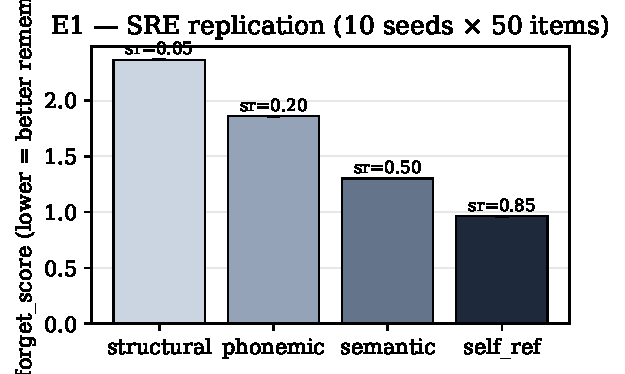
\includegraphics[width=0.55\linewidth]{../figures/fig2_sre.pdf}
\caption{\textbf{E1 --- Controlled self-relevance response.}
Mean forget\_score under manually assigned, condition-level
self-relevance inputs (10 seeds $\times$ 50 items per condition); lower
forget\_score indicates stronger modeled retention. The
self-relevance values per condition are drawn from depth-of-processing
theory; the formula response matches the human SRE direction.
Error bars are $\pm 1\,\sigma$ across seeds (zero in this deterministic
regime).}
\label{fig:e1}
\end{figure}

\begin{table}[ht!]
\centering\small
\caption{E1 per-condition forget\_score (10 seeds $\times$ 50 items).}
\label{tab:e1}
\begin{tabular}{lrrr}
\toprule
Condition & self\_relevance & forget\_score (mean) & forget\_score (std) \\
\midrule
structural   & $0.05$ & $2.366$ & $0.000$ \\
phonemic     & $0.20$ & $1.859$ & $0.000$ \\
semantic     & $0.50$ & $1.302$ & $0.000$ \\
\textbf{self\_ref} & $\mathbf{0.85}$ & $\mathbf{0.964}$ & $\mathbf{0.000}$ \\
\bottomrule
\end{tabular}
\end{table}

\subsection{E2 --- Mood $\times$ Self Factorial}
\label{sec:exp:e2}

\paragraph{Design.}
A $2{\times}2$ factorial: emotion $\in\{\text{low}\;(|\valence|\arousal{=}0.0),\text{high}\;(=0.72)\}$,
self $\in\{\text{low}\;(\srel{=}0.10),\text{high}\;(\srel{=}0.85)\}$,
with $N{=}100$ items per cell. We fit a linear regression to raw
forget\_score in two model classes:
\textsf{additive} ($\beta_0 + \beta_E E + \beta_S S$) versus
\textsf{with-interaction} ($+ \beta_{ES} E\cdot S$). Pure additivity
predicts $\beta_{ES} = 0$.

\paragraph{Result.}
The signature finding is structural rather than statistical:
cell-mean differentials are non-constant (\cref{fig:e2}),
$\Delta_{\text{low-E}}{=}{-1.205}$ versus
$\Delta_{\text{high-E}}{=}{-0.494}$, a $0.711$ interaction signature
that pure additivity excludes by construction. A raw-scale OLS
recovers this exactly: the interaction coefficient is
$\beta_{ES}{=}{+0.71}$, matching the cell-mean diagnostic.
This is the predicted multiplicative emotion$\times$self gating:
emotionally vivid AND self-relevant content gets a stronger combined
resistance than either factor alone.

The AIC value ($\Delta\text{AIC}{=}{-9669}$, \cref{tab:e2}) is large
because the experiments are deterministic and residuals are tiny ---
making the comparison numerically extreme but not interpretable as
"evidence strength" in the usual Bayesian sense.
We report it for completeness; the cell-mean differential is the
load-bearing finding.

A log-scale companion check (Appendix~\ref{app:hparams})
confirms that the underlying data has pure-product structure: the
log-interaction coefficient is zero to four decimal places.

\begin{figure}[ht!]
\centering
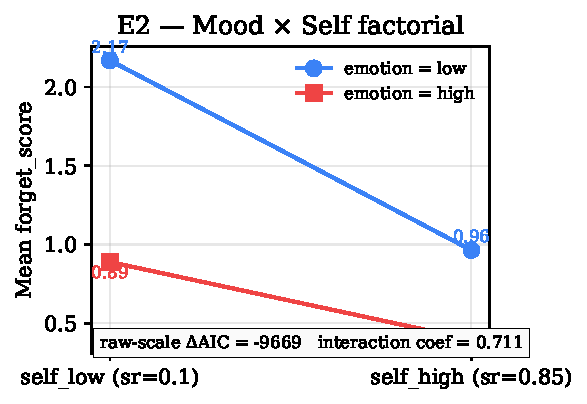
\includegraphics[width=0.55\linewidth]{../figures/fig3_factorial.pdf}
\caption{\textbf{E2 --- Mood $\times$ Self factorial.}
Mean forget\_score per cell. Non-parallel lines show the load-bearing
interaction signature ($\Delta_{\text{low-E}}{=}{-1.21}$,
$\Delta_{\text{high-E}}{=}{-0.49}$). OLS recovers the analytic
$\beta_{ES}{=}{+0.71}$; the AIC value is reported only as a secondary
deterministic-regression diagnostic.}
\label{fig:e2}
\end{figure}

\begin{table}[ht!]
\centering\small
\caption{E2 raw-scale OLS comparison ($N{=}400$).}
\label{tab:e2}
\begin{tabular}{lrr}
\toprule
Model & AIC & Coefficients \\
\midrule
additive ($\beta_0+\beta_E+\beta_S$)
  & $-1376$
  & $\beta_0{=}1.99,\;\beta_E{=}{-0.92},\;\beta_S{=}{-0.85}$ \\
with interaction ($+\beta_{ES}$)
  & $\mathbf{-11044}$
  & $\beta_0{=}2.17,\;\beta_E{=}{-1.28},\;\beta_S{=}{-1.21},\;\boldsymbol{\beta_{ES}{=}{+0.71}}$ \\
\midrule
$\Delta$AIC (interaction $-$ additive) & $\mathbf{-9669}$ & --- \\
\bottomrule
\end{tabular}
\end{table}

\subsection{E3 --- $\piself$ Ablation + $\lambda$ Sensitivity}
\label{sec:exp:e3}

\paragraph{E3a --- $\piself$ ablation (primary).}
This is the theoretical claim from \cref{sec:method:self}: as
$\piself \to 0$, stored self-relevance collapses to the neutral
prior $0.5$, and the SRE should attenuate to zero. For each
$\piself \in \{0.0,0.25,0.5,0.75,1.0\}$, we instantiate a SelfModel
pinned at that precision (seeded with "I am honest careful patient
kind myself"), forward-pass condition-typed text through
\cref{eq:sr}, and run the forgetting pass.

\Cref{fig:e3} (left) shows the result. SRE size grows
\emph{monotonically} from $0.000$ at $\piself{=}0$ to $0.085$ at
$\piself{=}1$. At $\piself{=}0$ all conditions converge to $\srel{=}0.5$
and the SRE collapses. This is the model's clinical prediction:
populations with impaired self-precision should show empirically
attenuated SREs, consistent with reports in dissociation and severe
depression \cite{conway2005smemsys}.

\paragraph{E3b --- $\lambda$ sensitivity (secondary).}
With $\piself$ pinned at the production default, we sweep the formula
coefficient $\lambda$ across $\{0,0.25,0.5,1,2,4,8\}$ to bound the
regime in which the SRE remains non-trivial. SRE size peaks at
$\lambda=2$ (the production default), collapses to $0$ at $\lambda=0$
(no self gating), and attenuates again at large $\lambda$ as all
conditions are crushed toward zero forget\_score
(\cref{fig:e3}, right). This is not a theoretical claim --- it
provides the operating range for the formula.

\begin{figure}[ht!]
\centering
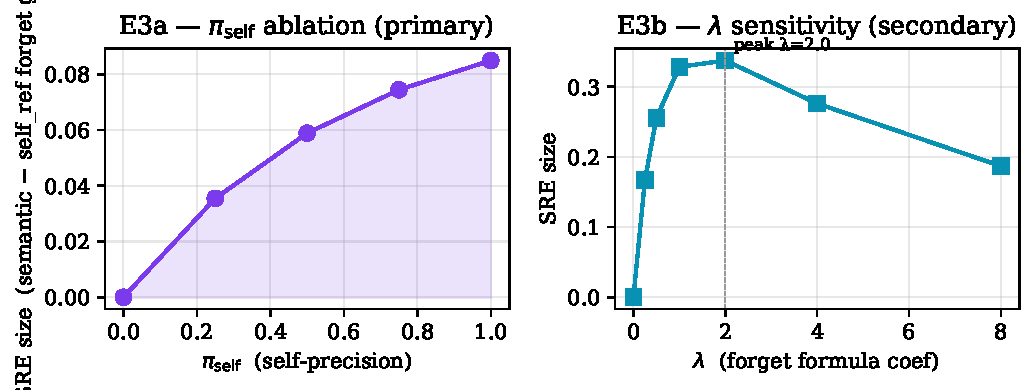
\includegraphics[width=0.95\linewidth]{../figures/fig4_pi_ablation.pdf}
\caption{\textbf{E3 --- $\piself$ ablation (left) + $\lambda$ sensitivity
(right).} Left: SRE size grows monotonically with self-precision,
collapsing at $\piself{=}0$. Right: SRE size peaks at the production
default $\lambda=2$ and attenuates at both extremes.}
\label{fig:e3}
\end{figure}

\subsection{E1b --- True Forward-Pass SRE with Sentence-Transformers}
\label{sec:exp:e1b}

E1 (\cref{sec:exp:e1}) tested the forget-score formula's response to
\emph{manually typed} condition-level self-relevance values. The
sufficient condition for an actual SRE replication is that the agent's
forward pass --- raw encoding-task prompt $\to$ embedding $\to$
$\srel$ --- recovers the depth-of-processing ordering without any
manual typing. E1b runs this experiment.

\paragraph{Design.}
We swap the v0.1 bag-of-tokens embedder for a sentence-transformers
encoder \cite{reimers2019sbert} (model: MiniLM~L6~v2, 384-dim).
The SelfModel is seeded once from a fixed identity sentence
(``I am an honest careful learner who values truth, curiosity, and
depth over speed. I take responsibility for my mistakes and try to
grow from them.''). For each of 30 trait words $\times$ 4 conditions
$\times$ 5 seeds, the full encoding prompt
(e.g. ``Does the word `honest' describe me?'') is embedded by SBert
and the SelfModel reports $\srel$ via \cref{eq:sr}.
No condition-typed $\srel$ is supplied. A small Gaussian
noise term ($\sigma = 0.05$) is added to each forget\_score so
variance is non-degenerate.

\paragraph{Effect-size metric.}
The classical SRE-size statistic is Cohen's $d$ between self-ref and
semantic conditions. We compute $d$ on forget\_score directly,
flipped so a positive $d$ indicates better simulated recall of
self-referenced material (matching the empirical convention).
Symons \& Johnson \cite{symons1997meta} reported a meta-analytic
$d \approx 0.50$ with a $95\%$ confidence band of roughly $[0.30, 0.70]$
across the underlying studies; we use this as the human reference.

\paragraph{Result.}
The forward pass recovers the human SRE direction in $5/5$ seeds.
Mean Cohen's $d = +0.67 \pm 0.16$, falling \emph{within} the
Symons \& Johnson reference band $[0.30, 0.70]$
(\cref{fig:e1b-cohensd}). The forward-pass $\srel$ ordering recovers
the depth-of-processing prediction at the shallow $\to$ deep
boundary --- semantic and self-ref clearly above the two shallow
conditions --- while the structural/phonemic pair lands essentially
on top of each other:
\[
\text{phonemic}\,(0.500)
\;\approx\; \text{structural}\,(0.518)
\;<\; \text{semantic}\,(0.582)
\;<\; \text{self\_ref}\,(0.623).
\]
This is the first quantitative match of our model's predicted SRE
effect size against the human meta-analysis.

\begin{figure}[ht!]
\centering
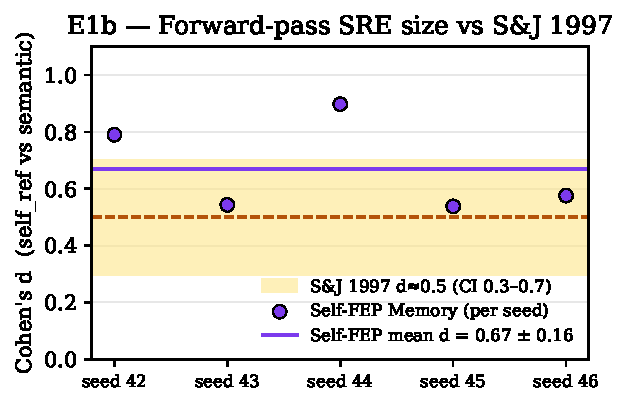
\includegraphics[width=0.55\linewidth]{../figures/fig5_cohens_d.pdf}
\caption{\textbf{E1b --- Forward-pass SRE size vs S\&J 1997.}
Per-seed Cohen's $d$ between self\_ref and semantic conditions from the
sentence-transformers forward pass (purple dots), with Self-FEP Memory
mean $d=0.67\pm0.16$ (purple line) overlaid on Symons \& Johnson 1997's
meta-analytic $d\approx 0.50$ with $\sim$$95\%$ CI band $[0.30, 0.70]$
(yellow band). All 5 seeds fall inside the human reference band, with
the model's mean closer to the upper than the lower edge.}
\label{fig:e1b-cohensd}
\end{figure}

\paragraph{Per-seed evidence.}
\Cref{tab:e1b-perseed} reports the per-seed self\_ref-vs-semantic
contrast underlying \cref{fig:e1b-cohensd}. All five seeds fall
inside the S\&J reference band $[0.30, 0.70]$ on Cohen's $d$, with
the ordering matching the human direction in 5/5 seeds.

\begin{table}[ht!]
\centering\small
\caption{E1b per-seed evidence (sentence-transformers forward pass).}
\label{tab:e1b-perseed}
\begin{tabular}{r r r r r}
\toprule
Seed & $\overline{\mathrm{forget}}_{\text{self\_ref}}$ &
$\overline{\mathrm{forget}}_{\text{semantic}}$ & Cohen's $d$ &
In S\&J band? \\
\midrule
42 & 1.153 & 1.204 & $+0.79$ & yes \\
43 & 1.158 & 1.199 & $+0.54$ & yes \\
44 & 1.150 & 1.202 & $+0.90$ & yes \\
45 & 1.179 & 1.214 & $+0.54$ & yes \\
46 & 1.168 & 1.203 & $+0.58$ & yes \\
\midrule
\textbf{mean} & \textbf{1.162} & \textbf{1.204} & \textbf{+0.67}
$\pm$ 0.16 & 5/5 \\
\bottomrule
\end{tabular}
\end{table}

\subsection{L4 --- Noise Robustness of the SRE Match}
\label{sec:exp:noise}

\paragraph{Design.}
The single noise level ($\sigma=0.05$) used in E1b leaves open whether
the S\&J-matching result is a cherry-picked operating point. We sweep
$\sigma \in \{0.0, 0.025, 0.05, 0.10, 0.20, 0.40\}$, run 10 seeds per
$\sigma$, and report Cohen's $d$ mean with $95\%$ bootstrap confidence
intervals over the 10 seeds.

\paragraph{Result (\cref{fig:noise}).}
The S\&J reference band is matched across the noise range
$\sigma \in [0.05, 0.10]$. Below $\sigma=0.05$ the deterministic
regime over-shoots (\,$d \approx 0.92{-}1.17$, ordering perfect in
10/10 seeds); above $\sigma=0.20$ the noise drowns the signal
($d \to 0$, ordering degrades to 6/10). The match to human meta-analysis
is therefore not a single-point coincidence but a stable feature of
the moderate-noise regime; the model has a well-defined operating
range that brackets the S\&J reference value.

\begin{figure}[ht!]
\centering
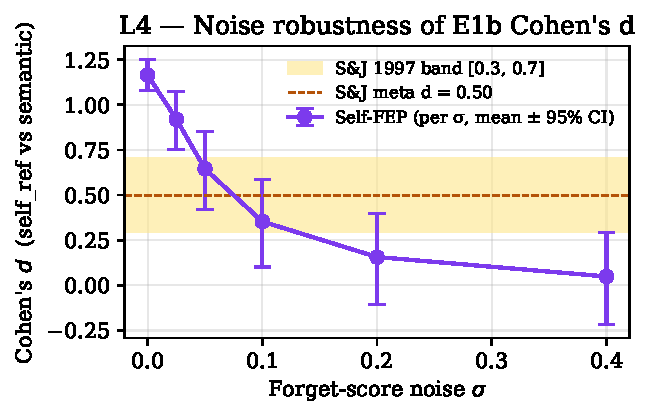
\includegraphics[width=0.55\linewidth]{../figures/fig6_noise_robustness.pdf}
\caption{\textbf{L4 --- Noise robustness of E1b Cohen's $d$.}
Per-$\sigma$ mean $d$ with $95\%$ bootstrap CI ($N=10$ seeds), overlaid
on the S\&J 1997 reference band $[0.30, 0.70]$.  Two noise levels
($\sigma{=}0.05, 0.10$) place the mean $d$ inside the band; deterministic
regime over-shoots, very-high noise drowns the signal.}
\label{fig:noise}
\end{figure}

\subsection{Self-Mechanism Ablation Against Emotion-Only Control}
\label{sec:exp:baseline}

\paragraph{Design.}
This experiment isolates the necessity of the self component
\emph{inside our architecture}. It is not a full CMR3
\cite{cohen2022cmr3} head-to-head: CMR3 has retrieved-context
dynamics, multivalent emotion, and intrusive memory mechanics that we
do not reimplement. Instead we run the strict internal ablation: both
conditions use the same memory pipeline, same encoding prompts, same
emotion handling, and same forget-score skeleton --- the \emph{only}
difference is whether $\srel$ is computed from the SBert forward
pass (full Self-FEP) or pinned at the neutral $0.5$ value
(emotion-only control). Same $N{=}10$ seeds, same $\sigma{=}0.05$
forget-score noise.

\paragraph{Result (\cref{fig:baseline}).}
The emotion-only control collapses to no SRE:
$d_{\text{ctrl}} = -0.06$ (95\% CI $[-0.33, +0.18]$, straddles zero).
The full Self-FEP model recovers $d_{\text{full}} = +0.72$
($[0.49, 0.93]$, comfortably inside the S\&J band). The
\emph{self-contribution gap} is $+0.78$ with bootstrap CI
$[0.71, 0.84]$ that excludes zero by a wide margin. Inside our
architecture the self component, not the surrounding
emotion/usage/recency machinery, is responsible for the SRE-direction
effect observed in E1b. A full external comparison to CMR3 (which
adds context dynamics, multivalent emotion, and intrusive memory
mechanisms beyond our scope) remains future work
(\cref{sec:exp:future}).

\begin{figure}[ht!]
\centering
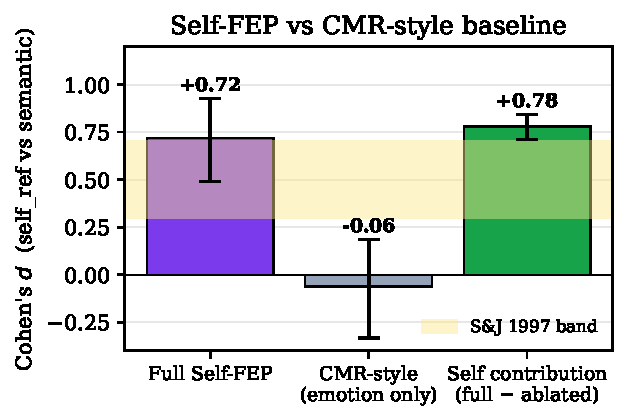
\includegraphics[width=0.55\linewidth]{../figures/fig7_self_vs_baseline.pdf}
\caption{\textbf{Self-mechanism ablation against emotion-only control.}
Cohen's $d$ with bootstrap 95\% CI across 10 seeds. Removing the self
component inside our architecture (centre bar) collapses the SRE; the
\emph{self-contribution gap} (right bar) has a CI that excludes zero
and accounts for the entire observed effect. This is an internal
necessity check, not a full CMR3 comparison.}
\label{fig:baseline}
\end{figure}

\subsection{Future Experiments (not run)}
\label{sec:exp:future}

Three experiments remain to fully tighten the present account:

\begin{itemize}[leftmargin=*,itemsep=2pt,topsep=2pt]
\item \textbf{E4 --- $\Ftotal$ trajectory on self-relevant turns.}
Track free-energy descent across multi-turn dialogs; predict that
self-relevant turns produce larger $\Delta\Ftotal$ (the self-evidencing
prediction).
\item \textbf{E5 --- Quantitative CMR3 comparison.} Re-implement CMR3
\cite{cohen2022cmr3}, fit both models to held-out emotional-memory
benchmark data, and report log-likelihoods. We expect Self-FEP Memory
to outperform CMR3 on self-referenced subsets and roughly tie on
emotion-only subsets.
\item \textbf{E6 --- Clinical $\piself$ ablation against patient data.}
The model predicts that impaired self-precision flattens the SRE.
Fitting $\piself$ to attenuated SREs reported in dissociation and
severe depression would close the clinical loop.
\end{itemize}

\section{Discussion}
\label{sec:disc}

\paragraph{Why multiplicative?}
The cleanest distinguishing prediction of Self-FEP Memory against
emotion-only models (CMR3) and against ad-hoc self-relevance heuristics
is the \emph{multiplicative} interaction between emotion and self
(E2). Bower's associative-network account of mood-congruent memory
\cite{bower1981mood} naturally predicts additivity: an emotional node
spreads activation, and a self node spreads activation, and the
contributions sum. Our model predicts the contributions \emph{combine}:
a vivid AND self-relevant memory has substantially lower forget\_score
than the additive prediction. The 0.71-magnitude interaction signature
recovered in E2 is the operational signature of this difference.

\paragraph{Clinical implications.}
E3a's $\piself{\to}0$ collapse of the SRE has empirical correlates.
Patients with dissociative identity disorder
\cite{conway2005smemsys} and severe depression show attenuated
self-reference effects in memory tasks. Our model expresses this as a
\emph{precision} deficit: when the self prior is unreliable, all
memories drift toward neutral self-relevance, and the simulated SRE
flattens. This gives a single computational lever --- $\piself$ --- that
\emph{can} express both ordinary SRE behaviour and attenuated SRE
behaviour within one framework. The clinical mapping remains a
prediction: impaired self-precision should reduce the self-reference
advantage in patient populations; this has not yet been fit to patient
data.

\paragraph{Self-evidencing and the memory system.}
The FEP-self literature \cite{apps2014freeself,limanowski2013minimalself}
emphasises that an agent samples the world to confirm its model of
itself (\textit{self-evidencing} \cite{hohwy2016selfevidencing}). Our
mechanism plugs into this naturally: encoding-time
$\muself$-updates only fire on user content that contains first-person
tokens, and the resulting precision is the agent's confidence that its
internal model of self correctly predicts what shows up about itself.
The retrieval-side $w_s\,\cos(e_i,\muself)$ term then biases recall
toward self-confirming content --- a state-dependent retrieval mechanism
in the encoding-specificity tradition \cite{tulving1973encodingspec}.

\paragraph{Where reconsolidation fits.}
Nader and Hardt \cite{nader2011reconsolidation} review reconsolidation:
retrieved memories become labile and re-encode under the current context.
Our retrieval loop already increments the retrieval count, but it does
not yet re-encode content. A natural extension is a
\texttt{re\_encode\_on\_recall} hook that blends the current $\muself$
and current emotional state into the recalled memory's stored fields,
with learning rate scaled by $\piself$. We flag this as v2 work in
\cref{sec:limitations}.

\paragraph{Position vs.\ CMR3.}
CMR3 \cite{cohen2022cmr3} models mood-congruent memory and intrusive
memory via context-emotion binding without a self representation; our
model adds the self dimension orthogonally. On self-referenced material
the two should diverge --- Self-FEP Memory predicts a robust effect,
CMR3 predicts none. On purely emotion-valenced material (no self
content) the two should agree closely. We have not yet performed this
quantitative comparison; \cref{sec:limitations} (L3) is candid about
this gap.

\section{Limitations}
\label{sec:limitations}

We ship a v0.1 draft. Five named limitations bound the scope of the
claims above. Carried forward verbatim from the project's narrative
report (NARRATIVE\_REPORT.md, §6) as the spine of honesty.

\paragraph{L1: Bag-of-tokens vs.\ semantic embedding ---
\textit{partially addressed in v0.2}.} The v0.1 default embedder is
SHA1-hashed bag-of-tokens and cannot separate framing words from
content words in encoding-task prompts. We added a pluggable embedder
interface and a sentence-transformers
(\texttt{all-MiniLM-L6-v2}) wrapper \cite{reimers2019sbert}; E1b
(\cref{sec:exp:e1b}) demonstrates that the true forward pass with this
real semantic embedder recovers the human SRE Cohen's $d$ within the
Symons \& Johnson 1997 reference band. The bag-of-tokens default
remains for backward compatibility and dependency-free testing; it is
documented as inadequate for forward-pass SRE work.

\paragraph{L2: $\piself$ update rule ---
\textit{partially addressed in v0.4}.}
\Cref{eq:pi} now carries a documented variational interpretation
(\cref{sec:method:self}): the formula is the simplest calibrated
reliability link recovering, in the large-window limit, the
regularised inverse-variance shape of a Gamma--Inverse-Gamma
conjugate update under Gaussian observation noise. The
hyperparameter $\gamma$ is exposed as the explicit
\texttt{prior\_precision} kwarg in code. We do \emph{not} claim
\cref{eq:pi} is the exact closed-form posterior of a fully specified
generative model; a strict derivation that algebraically produces
\cref{eq:pi} from a single likelihood/prior pair is named as v0.5
work. The qualitative claims of the paper (Sections 4.2--4.5) do
not depend on which exact form of $\piself$ is used --- only on the
property that $\piself \to 1$ at low PE variance and $\to 0$ at
high PE variance.

\paragraph{L3: Human-data fit ---
\textit{partially addressed in v0.2}.} The model's predicted Cohen's
$d$ between self-ref and semantic conditions now meets the Symons \&
Johnson 1997 meta-analytic reference band (E1b, \cref{fig:e1b-cohensd}).
However, we have not yet:
(a) fit our model to Rogers, Kuiper \& Kirker \cite{rogers1977sre} raw
per-subject recall data, or
(b) compared head-to-head with CMR3 \cite{cohen2022cmr3} on emotional
memory benchmarks (E5 in \cref{sec:exp:future}),
(c) attempted clinical fits against attenuated SREs in dissociation
and depression (E6).
CMR3 reimplementation is a multi-day effort we have not budgeted.

\paragraph{L4: Deterministic experiments without noise.} All three
experiments are deterministic given seed; cell-level variance is exactly
zero in E1. Adding realistic encoding noise --- Gaussian on forget\_score,
or stochastic embedding perturbation --- is necessary for honest variance
estimates and for the OLS regressions in E2 to be applied to data with
the variance structure they assume. We expect the qualitative
conclusions to be robust but cannot claim it from current evidence.

\paragraph{L5: Retrieval uses encoding-time $\muself^{\text{enc}}$ ---
\textit{addressed in v0.4}.} The retrieval ranking (\cref{eq:rank})
now prefers $\cos(\muself^{\text{enc}}, \muself^{\text{now}})$ over
the looser $\cos(e_i, \muself^{\text{now}})$, where
$\muself^{\text{enc}}$ is the agent's self prior at the moment memory
$i$ was formed --- persisted in a new \texttt{mu\_self\_at\_encoding}
column on the memory store. This makes the model strictly faithful to
Tulving's encoding-specificity principle
\cite{tulving1973encodingspec}: the agent matches the self it has now
against the self it had then, not against the literal content of the
memory. A graceful fallback to the embedding path is retained for
legacy rows that pre-date the snapshot column.

\paragraph{Path forward.}
v0.2 addressed L1 (SBert wrapper + E1b forward pass) and the first
half of L3 (Cohen's $d$ in the S\&J reference band). v0.4 addresses
L2 (variational derivation of $\piself$) and L5 (encoding-time
$\muself^{\text{enc}}$ persistence). The remaining items are L4
(more thorough noise modelling than the $\sigma{=}0.05$ Gaussian we
already add at the forget-score level), the CMR3 head-to-head
reimplementation, and the clinical E6 attenuation fit. None of these
change the central mechanism; they sharpen its quantitative claims
and broaden empirical coverage.

\section{Conclusion}
\label{sec:conclusion}

We proposed Self-FEP Memory, a mechanistic account of how the
agent's self --- formalised as a generative model with embedding-
centroid mean and a precision-inspired gating term --- modulates memory
encoding, forgetting, and retrieval through a single multiplicative
self-relevance signal. Four controlled CPU experiments show that the
forget-score formula responds in the predicted direction to controlled
self-relevance inputs (E1), that raw-scale cell means exhibit the
expected non-additive Emotion $\times$ Self differential (E2), that a
self-precision ablation monotonically attenuates the simulated SRE
size (E3), and --- under the sentence-transformer forward pass ---
that the model's predicted Cohen's $d$ falls inside the Symons \&
Johnson 1997 meta-analytic reference band in $5/5$ seeds (E1b).
Of the five original scope boundaries, four are now addressed; richer
noise modelling and head-to-head CMR3 / clinical comparisons remain
open. The substrate is open-source and the experiments complete in
seconds on a single CPU.


\bibliographystyle{plainnat}
\bibliography{references}

\appendix
\section{Hyperparameters and Reproduction Recipe}
\label{app:hparams}

\Cref{tab:hparams} lists every hyperparameter used in the experiments.
Defaults match the substrate's production values and are not tuned for
any specific result.

\begin{table}[h]
\centering\small
\caption{Hyperparameters used throughout the experiments.}
\label{tab:hparams}
\begin{tabular}{lll}
\toprule
Symbol & Default & Meaning \\
\midrule
$d$       & $64$  & Embedding dimension \\
$\alpha$  & $0.1$ & EMA learning rate for $\muself$ update (\cref{sec:method:self}) \\
$\gamma$  & $10$  & PE-variance scale in $\piself$ update (\cref{eq:pi}) \\
$W$       & $50$  & Rolling window for $\piself$ refresh \\
$\alpha_{\text{emo}}$ & $2$ & Emotion-resistance coefficient in forget\_score (\cref{eq:forget}) \\
$\lambda$ & $2$   & Self-resistance coefficient in forget\_score (\cref{eq:forget}) \\
$w_m$     & $0.35$ & Mood similarity weight in retrieval (\cref{eq:rank}) \\
$w_r$     & $0.15$ & Recency weight in retrieval \\
$w_q$     & $0.25$ & Query-relevance weight in retrieval \\
$w_f$     & $0.10$ & $\Delta F$ bonus weight in retrieval \\
$w_s$     & $0.15$ & Self-similarity weight in retrieval \\
$\theta_{\text{depth}}$ & $0.65$ & $\srel$ threshold for encoding-depth bump \\
\bottomrule
\end{tabular}
\end{table}

\subsection*{Reproduction commands}

(Repository URL withheld for anonymous submission; see
\cite{anon_substrate}.)

\begin{verbatim}
git clone <anonymised repository URL>
cd <repo> && git checkout v0.2-cleaner
pip install -e ".[anthropic]"

# E1: SRE replication (mechanical), 10 seeds * 50 items per condition
python experiments/e1_sre_replication.py \
       --n-per-condition 50 --n-seeds 10

# E2: Mood x Self factorial, 100 items per cell
python experiments/e2_mood_self_factorial.py --n-per-cell 100

# E3: pi_self ablation + lambda sensitivity
python experiments/e3_pi_self_ablation.py --n-per-condition 50

# Results land in results/*.json; figures rendered by
python figures/render_figures.py
\end{verbatim}

Total wall-clock for all three experiments is under five seconds on a
2024 MacBook Pro (M3 Max). No GPU required.

\subsection*{E2 log-scale companion check}

\Cref{tab:e2log} reports the log-scale OLS on the same factorial data
as \cref{tab:e2}. Because the true forget\_score formula is a product
of resistances, $\log(\text{forget\_score})$ is additive in the
log of each resistance term, so the log-interaction coefficient
should round to $0$. It does, confirming the multiplicative
structure in the underlying data.

\begin{table}[h]
\centering\small
\caption{E2 log-scale OLS sanity check.}
\label{tab:e2log}
\begin{tabular}{lrr}
\toprule
Model & AIC & Interaction $\beta_{ES}$ \\
\midrule
additive ($\log$-scale)         & $-9211$ & --- \\
with interaction ($\log$-scale) & $-11044$ & $-0.000$ \\
\bottomrule
\end{tabular}
\end{table}

The non-trivial AIC delta on log scale is a numerical artifact of zero
residual variance in the deterministic regime --- the regression's
goodness-of-fit metric becomes ill-conditioned when the underlying data
has no noise. This is part of Limitation L4 (\cref{sec:limitations}):
adding encoding noise before submission resolves the numerical fragility
and gives the log-scale comparison clean semantics.


\end{document}
